\section{\bf Examples}

\subsection{Classical Mechanics}
\begin{frame}
    \frametitle{Classical Mechanics I}
    We recover Classical Mechanics by taking the bundle 
    $$\mathbb{R} \times Q \xrightarrow{\pi} \mathbb{R}.$$ 
    Then, a section is just a curve $\gamma: \mathbb{R} \rightarrow Q.$
    \begin{center}
        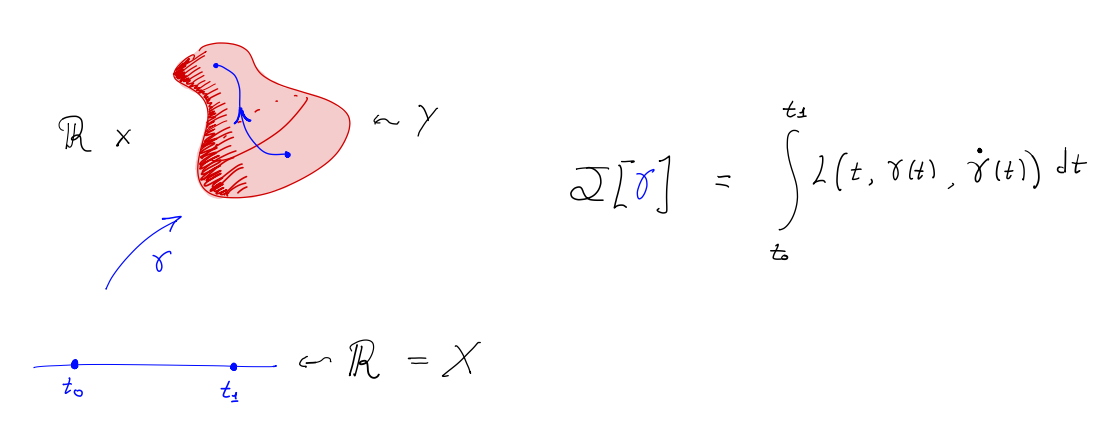
\includegraphics[width = 300pt]{Images/Classical_Mechanics.PNG}
    \end{center}
\end{frame}

\begin{frame}
    \frametitle{Classical Mechanics II}
    The jet bundle:
    $$J^1 \pi = \mathbb{R} \times TQ,$$
    and the \alert{Poincaré-Cartan} form fixed a Lagrangian (which will be identified with a function) $$L : \mathbb{R} \times TQ \rightarrow \mathbb{R}$$ is 
    $$\theta_L = \pdv{L}{\dot{q}^i}d \dot{q}^i - \left(\pdv{L}{\dot{q}^i} \dot{q}^i - L \right) dt.$$
    Dyanmics are vector fields $X$ satisfying 
    \begin{itemize}
        \item \textit{Stationary condition}, $\iota_X d \theta_L = 0.$
        \item \textit{Normalization}, $dt(X) = 1.$
    \end{itemize}
    We recover \alert{cosymplectic} geometry!
\end{frame}

\begin{frame}
    \frametitle{Classical Mechanics III}
    What about Noether Theorem?
    Suppose $L$ $t$-invariant. Then, time translations $\pdv{t}$ define a symmetry of the corresponding multisymplectic form.
    Hence, by previous considerations, $\iota_{\pdv{t}} \theta_L$ is an \alert{conserved current}, that is, a \alert{conserved quantity}.  
    Locally, $$\iota_{\pdv{t}} \theta_L = \pdv{L}{\dot{q}^i} \dot{q}^i - L = H,$$
    obtaining conservation of energy.
\end{frame}

\subsection{Hyperelastic materials}
\begin{frame}
    \frametitle{Hyperelastic materials I}
    We will give an example of hyperelastic dynamics in a fixed background.
    \begin{itemize}
        \item Fix a \alert{body} $(B, G), \rho$, where $B$ is a smooth manifold, $G$ is a Riemannian metric on $B$, and $\rho$ is the mass density.
        \item Fix a background manifold $(M, g)$, with $M$ a smooth manifold and $g$ a Riemannian metric on $B$.
    \end{itemize}
    Dynamics of $B$ on $M$ are time-dependent embeddings $$\phi_t : B \rightarrow M.$$
    We model these embeedings as \alert{fields} $$Y \xrightarrow{\pi} X.$$
\end{frame}

\begin{frame}
    \frametitle{Hyperelastic materials II}
    \begin{itemize}
        \item $X := \mathbb{R} \times B.$
        \item $Y := \mathbb{R} \times B \times M.$
        \item The \alert{projection} $\pi$ is the trivial choice.
    \end{itemize}
    
    There is an \alert{issue}:
    \begin{itemize}
        \item Arbitrary fields of the previous bundle $\phi: X \rightarrow Y$ \textit{do not} necessarily correspond to
        time-dependent embeddings.
    \end{itemize}
    But not for long... 
    \begin{itemize}
        \item Nevertheless, we can still apply the theory developed because embeddings are stable under local perturbations (variations).
    \end{itemize}
\end{frame}

\begin{frame}
    \frametitle{Hyperelastic materials III}
    \begin{center}
        {\large \bf What is the \alert{Lagrangian}?}
    \end{center}
    \alert{Notation}:
    \begin{itemize}
        \item Coordinates on $B$ are denoted by $(x^i) = x^1, \dots, x^{n-1}.$
        \item When adding the time coordinate $t = x^0$, we get coordinates $(x^\mu)$ on $X$.
        \item Coordinates on $M$ are denoted by $(y^a)$.
    \end{itemize}
    Then, the \alert{Lagrangian} is:
    \begin{align*}
        \mathcal{L} &= \mathbb{K} - \mathbb{P}\\
        &= \frac{1}{2} \sqrt{\det G} \rho g_{ab} z^a_0 z^b_0 d^{n+1}x
        - \sqrt{\det G}\rho W(x^\mu, G, g, z^a_i) d^{n+1}x,
    \end{align*}
    where $W$ is the stored energy.
\end{frame}

\begin{frame}
    \frametitle{Hyperelastic materials IV}
    The \alert{Poincaré-Cartan} form is 
    \begin{align*}
        \Theta_\mathcal{L} &= \rho g_{ab}z^b_0 \sqrt{\det G} dy^a \wedge d^n x_0 - \rho \pdv{V}{z^a_i} \sqrt{\det G} dy^a \wedge d^nx_i\\
        & - \left(-\pdv{W}{z^a_i} z^a_i + \frac{1}{2} g_{ab}z^a_0z^b_0 + W\right) \rho \sqrt{\det G} d^{n+1}x
    \end{align*}
    How can we apply Noether's Theorem?
    \begin{itemize}
        \item There is a clear symmetry, \alert{time-invariance}.
        \item Then, the current obtained through the theory is
        \begin{align*}
            \alpha &= -\rho \pdv{W}{z^a_i} \sqrt{\det G} dy^i d^n x_{i0}\\
             &+ \left(\frac{1}{2}g_{ab}z^a_0z^b_0  + W - \pdv{W}{z^a_i} z^a_i\right) \rho \sqrt{\det G} d^{n+1} x_0.
        \end{align*}
    \end{itemize}
\end{frame}

\begin{frame}
    \frametitle{Hyperelastic materials V}
    on holonomic sections it takes the expression
    $$\alpha =\left(  \frac{1}{2} g_{ab}z^a_0z^b_0 + W \right)\rho \sqrt{\det G} d^{n+1} x_0 + \rho \pdv{W}{z^a_i}z^a_0 \sqrt{\det G} d^n x_i$$
    Since $$e = \left(  \frac{1}{2} g_{ab}z^a_0z^b_0 + W \right)\rho \sqrt{\det G}d^{n+1}x_0$$ can be though of as the \alert{energy dentisy}.
    This gives us a conservation law, where $$\rho \pdv{W}{z^a_i}z^a_0 \sqrt{\det G} d^n x_i$$ is the energy flux.
\end{frame}

\begin{frame}
    \frametitle{Final remarks}
    \begin{itemize}
        \item Multisymplectic geometry is a tool that allows us to study variational problems (field theory, Classical Mechanics, 
        some problems in material modelling...)
        \item It is a very active area of research, both from the mathematical and the physical point of view.
        \item Applications to material modelling seem interesnting, have been practically unexplored.
    \end{itemize}
\end{frame}

\begin{frame}
    \nocite{*}
    \printbibliography
\end{frame}

\begin{frame}[plain]
    \begin{center}
        {\Large Thank you for your attention!}
    \end{center}
\end{frame}

